\section{Etape 1}
\subsection{Objectifs}

L'objectif de ce projet fil rouge est de permettre la mise en place d'une infrastructure de communication.
Il nous permettra de découvrir, étudier et mettre en place différents protocoles de communication. Cette première étape
consiste à faire passer une information entre une source et une destination en utilisant
un transmetteur parfait. Grâce à cela, nous découvrirons l'architecture logicielle proposée pour ce projet. Nous en profiterons également.
Pour commencer la mise en place de test utilisant JUnit afin d'assurer le fonctionnement des différents composants du système.

\subsection{Choix d'implémentation}

Pour permettre une utilisation simple et rapide du simulateur, la mise en place de scripts de compilation, de création de documentation et d'éxécution
ont été mis en place. Ces scripts sont disponibles à la racine du projet.
Il est donc possible de compiler puis tester le simulateur en utilisant les divers arguments spécifiés dans le readme.

Les différentes fonctionnalitées implémentées dans l'étape 1 (transmetteur parfait) sont les suivantes:
nbsample

En prévision d'une potentielle fusion de binômes, nous avons décidé de mettre en place une architecture logicielle versionné sur git.
Elle nous permettra à chacun de reprendre le projet et de travailler sur des fonctionnalitées différentes sans avoir à se soucier des conflits de version.

\pagebreak

\subsection{Sondes}

Lors de l'execution de la commande: 

\begin{figure}[h]
    \centering
    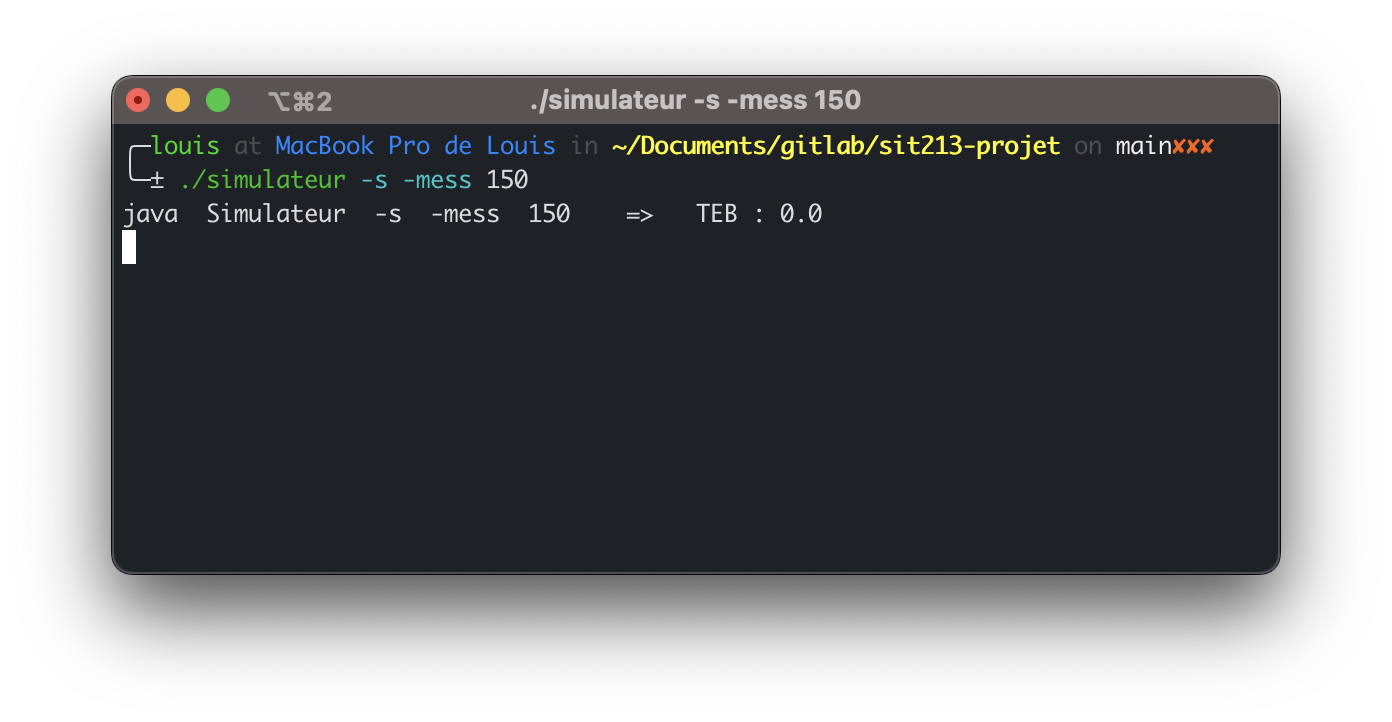
\includegraphics[width=\textwidth]{term_1.png}
    \caption{terminal}
\end{figure}

On constate lors de l'execution du script l'affichacge d'un signal identique sur la source et la destination (voir figure 2). Cela coincide 
avec le fait que le transmetteur est parfait et que le signal n'est donc pas modifié lors de la transmission vers la destination.
Le TEB est égal à 0 comme attendu.

\begin{figure}[h]
    \centering
    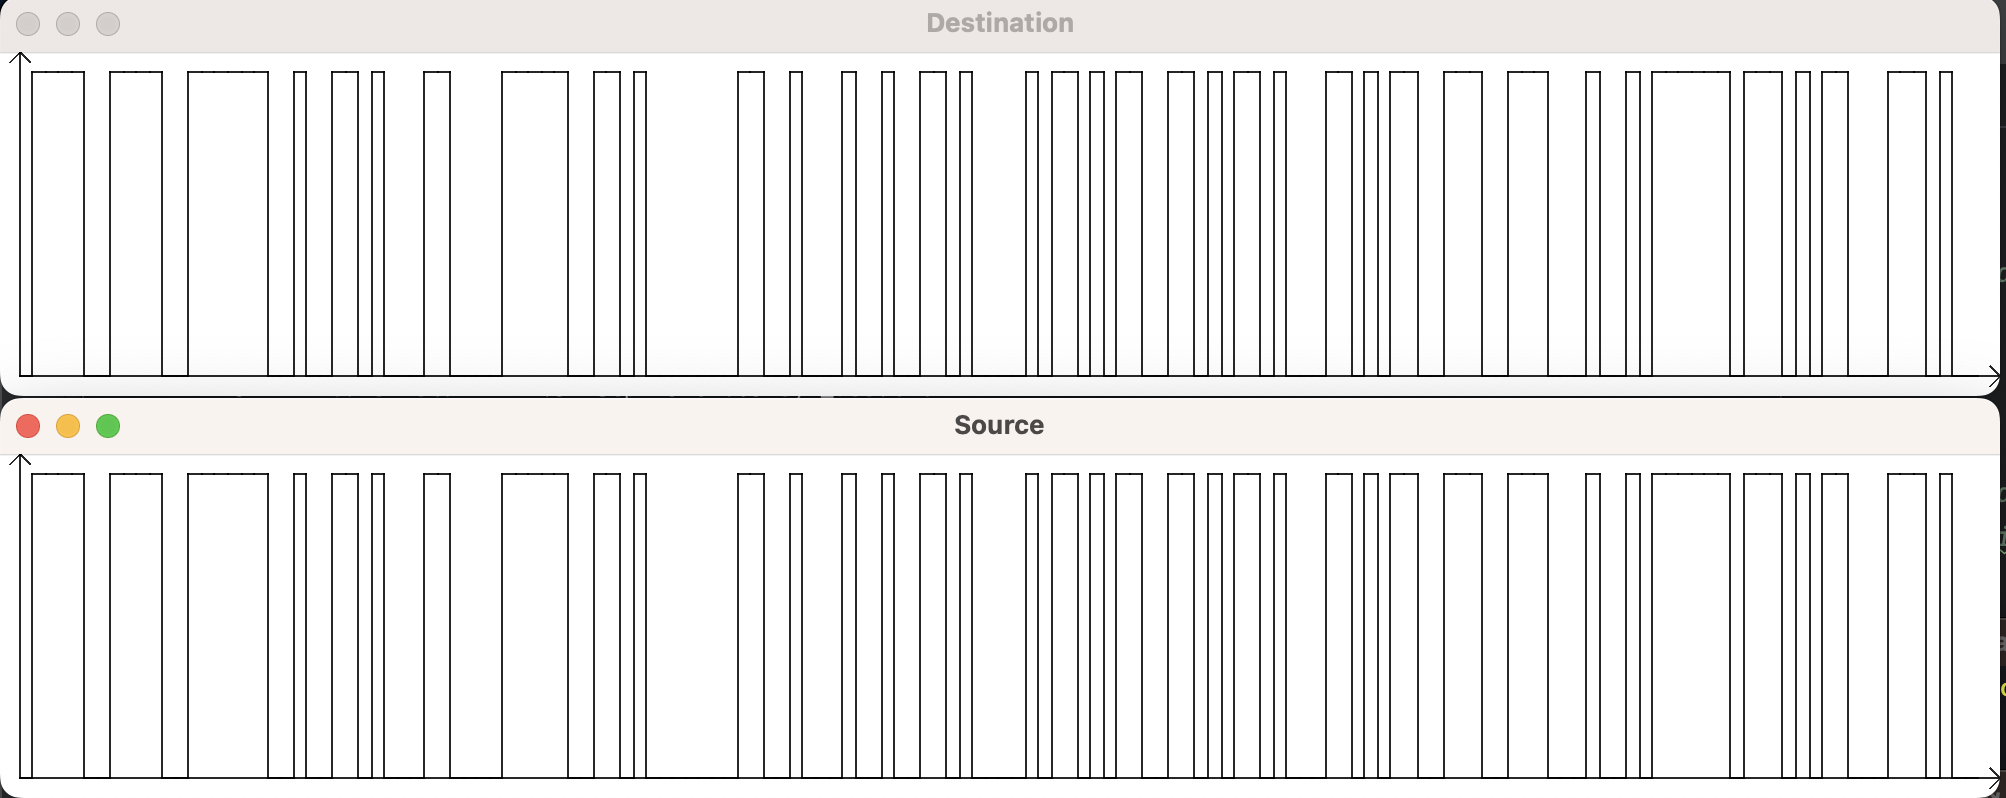
\includegraphics[width=\textwidth]{s_r_100.png}
    \caption{Execution du programme}
\end{figure}

\pagebreak

Executer le programme deux fois en utilisant la meme graine nous permet d'obtenir la meme génération de signal.
Cela nous sera utile dans le cadre de tests ultérieurs afin de s'assurer du bon fonctionnement du simulateur dans plusieurs situations différentes.

\begin{figure}[h]
    \centering
    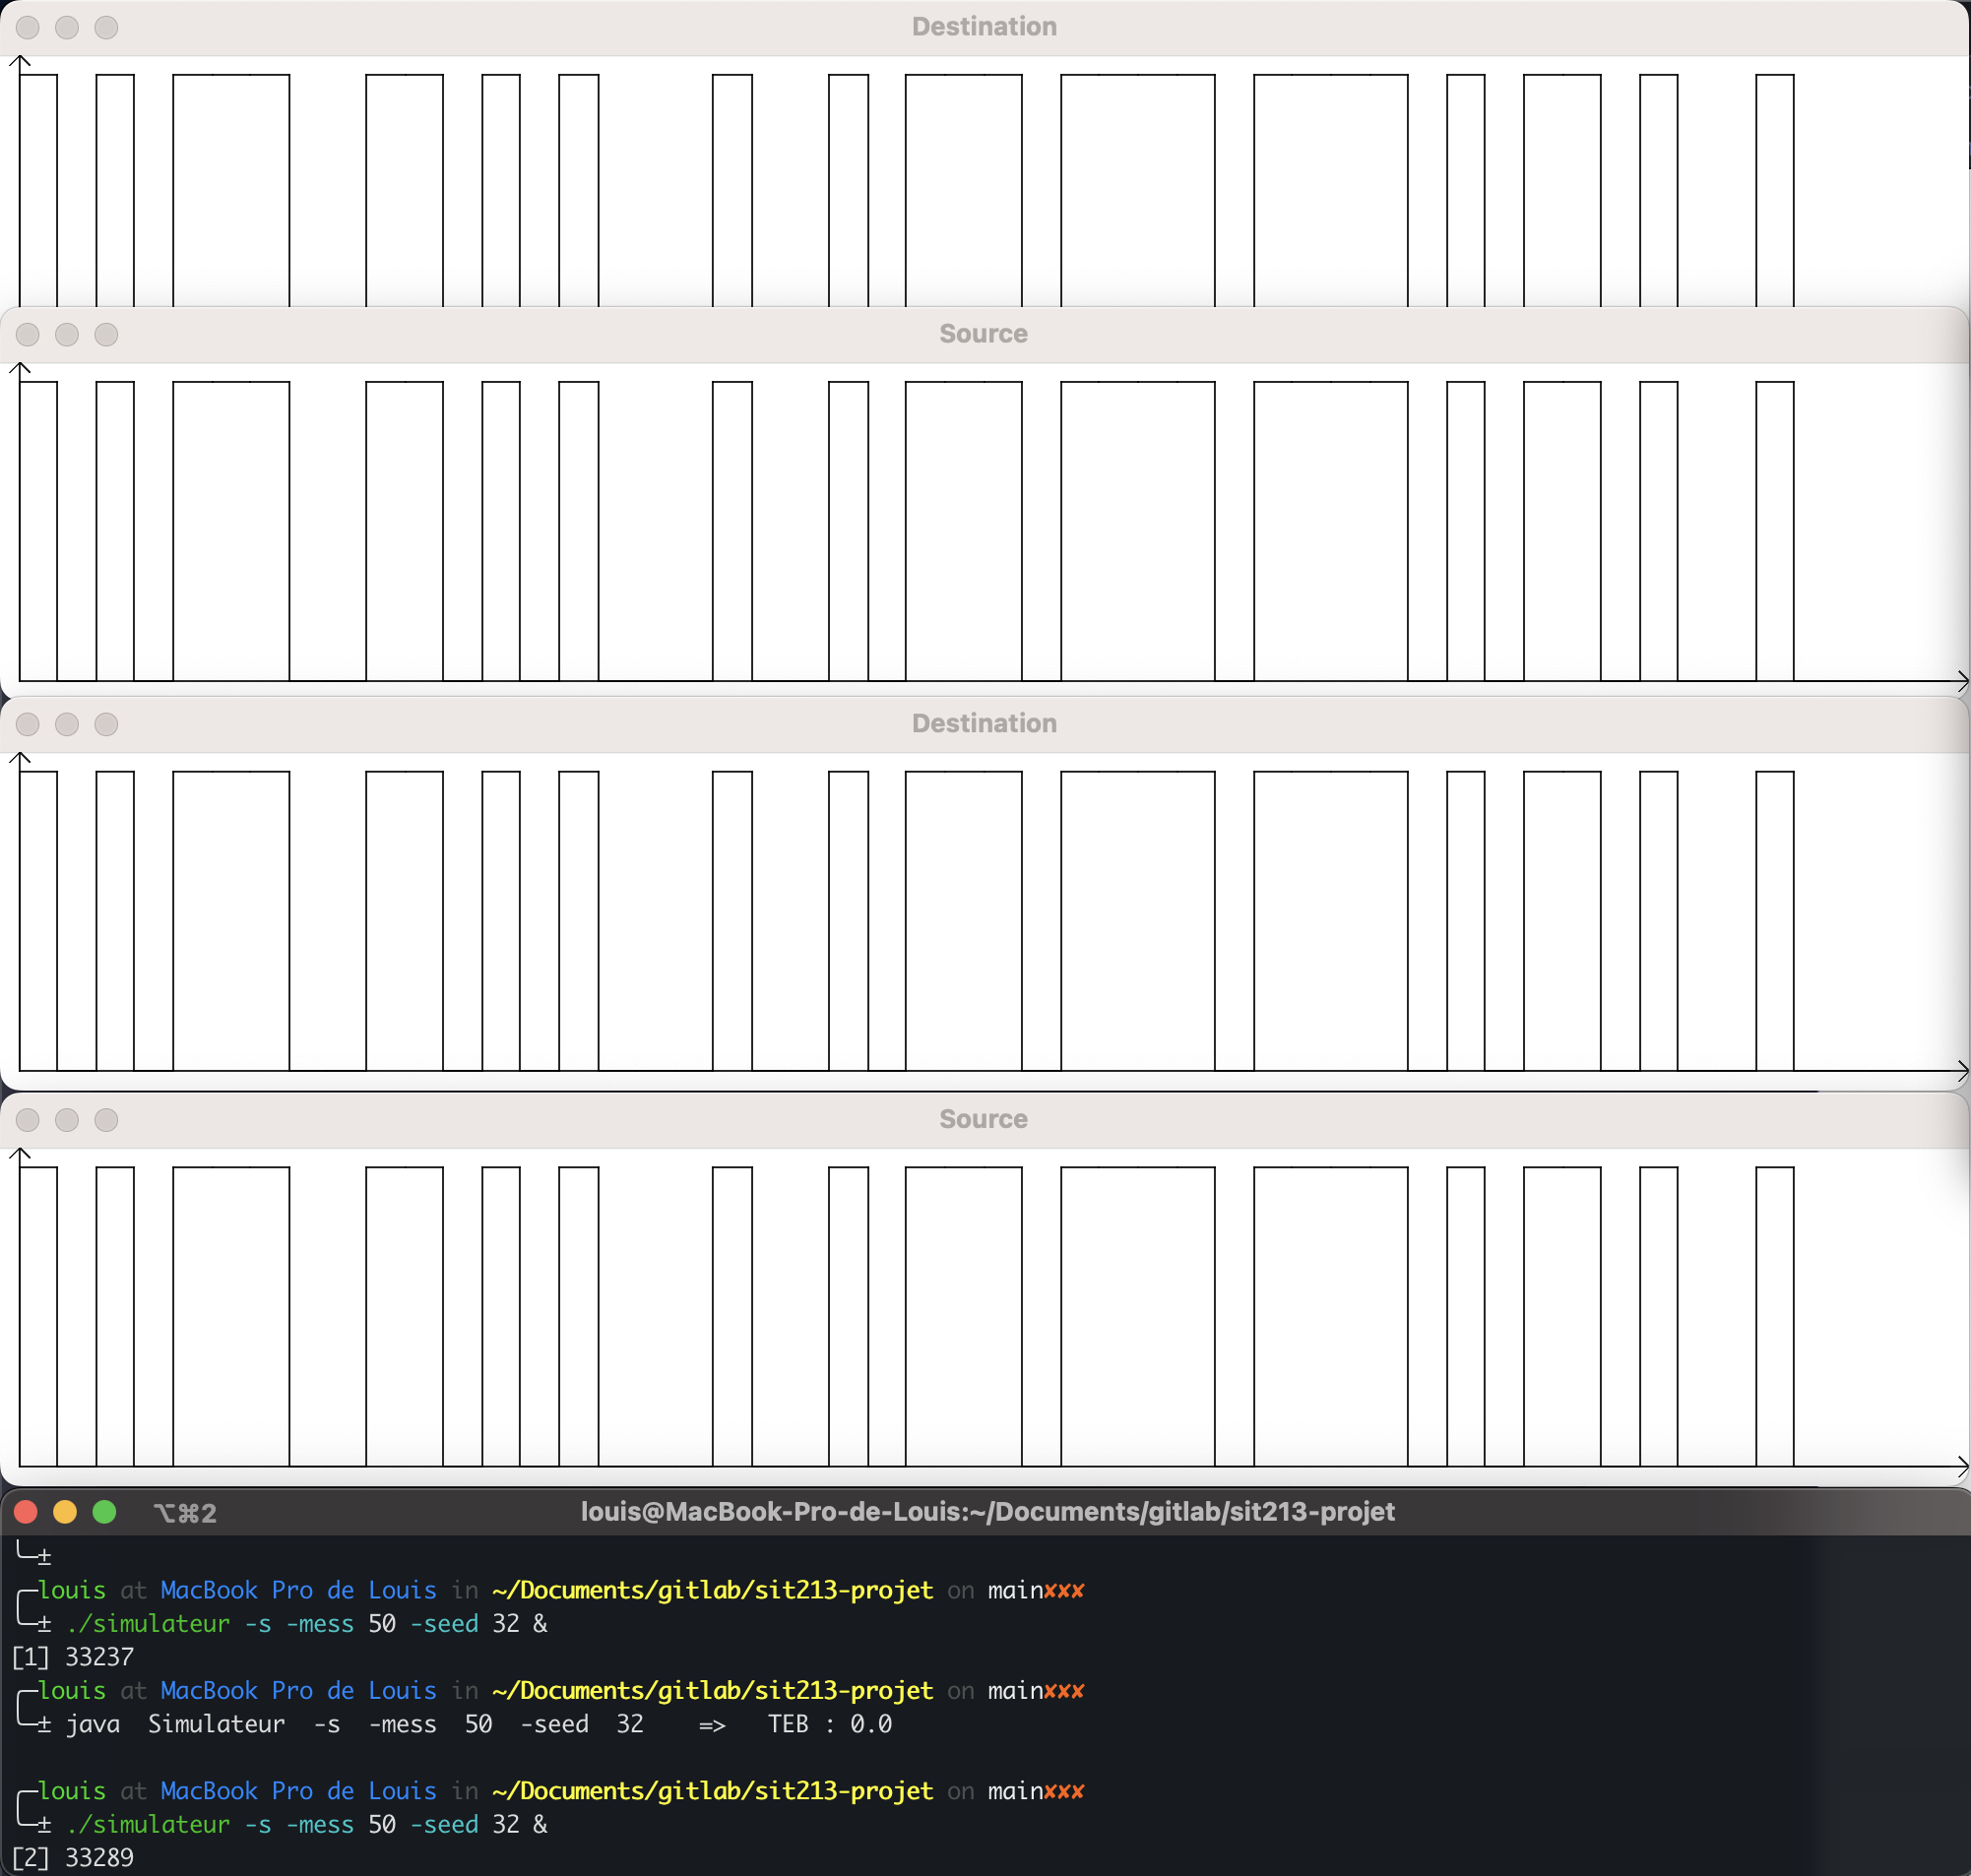
\includegraphics[width=\textwidth]{s_r_50.png}
    \caption{Exemple utilisation d'une "seed"}
\end{figure}

% \subsection{Performances}

\subsection{Conclusion}

Cette première étape a été très utile dans la compréhension de l'architecture logicielle mise à disposition.
Cela aura été l'occasion de commencer à penser à l'organisation du travail d'équipe à venir et de mettre en place des outils de travail collaboratif.


